\section{Học Tự giám sát (Self-Supervised Learning)}
\label{sec:self_supervised_learning}

\subsection{Tổng quan: Giải phóng AI khỏi Xiềng xích của Nhãn}
\label{subsec:ssl_overview}
Trong thế giới lý tưởng, chúng ta có một nguồn cung cấp vô tận dữ liệu được gán nhãn cẩn thận để huấn luyện các mô hình ngày càng lớn hơn. Nhưng trong thực tế, dữ liệu có nhãn là một tài nguyên khan hiếm, đắt đỏ và tốn thời gian để tạo ra. Ngược lại, dữ liệu không nhãn—hàng tỷ bức ảnh trên internet, hàng giờ video được tải lên mỗi phút—lại gần như vô tận. \textbf{Học Tự giám sát (Self-Supervised Learning - SSL)} ra đời như một câu trả lời cho nghịch lý này.

\textbf{Định nghĩa:} SSL là một phương pháp học máy trong đó mô hình học các biểu diễn (representations) hữu ích từ dữ liệu không nhãn bằng cách tự tạo ra các "tín hiệu giám sát" (supervisory signals) từ chính dữ liệu đó. Thay vì học từ các nhãn do con người cung cấp (ví dụ: "con mèo", "con chó"), mô hình được giao một \textbf{nhiệm vụ giả (pretext task)} mà lời giải đã có sẵn trong dữ liệu đầu vào.

\begin{mdframed}[style=infobox]
	\textbf{Trực giác của Pretext Task}
	
	Hãy tưởng tượng bạn đưa cho một AI một bức ảnh ghép hình (jigsaw puzzle) đã bị xáo trộn và yêu cầu nó sắp xếp lại. Để giải quyết nhiệm vụ này, AI không cần biết các mảnh ghép đó là của một "con mèo" hay "tòa nhà". Thay vào đó, nó buộc phải học về các quy luật thị giác cơ bản: các đường viền nối tiếp nhau như thế nào, các mảng kết cấu khớp nhau ra sao, và các bộ phận của một vật thể thường có mối quan hệ không gian như thế nào.
	
	Thông qua việc giải quyết bài toán giả này, AI đã tự học được một biểu diễn phong phú về thế giới thị giác. Biểu diễn này, sau đó, có thể được tinh chỉnh (fine-tuned) một cách dễ dàng cho các tác vụ xuôi dòng (downstream tasks) như phân loại hay phát hiện vật thể, thường chỉ với một lượng nhỏ dữ liệu có nhãn.
\end{mdframed}

Mục tiêu cuối cùng của SSL là huấn luyện trước (pre-train) một bộ mã hóa đặc trưng (feature encoder) mạnh mẽ. Một encoder được huấn luyện tốt bằng SSL có thể được xem như một "xương sống thị giác" đa năng, nắm bắt được "ngữ pháp" của hình ảnh, sẵn sàng để áp dụng cho nhiều bài toán khác nhau. Có hai trường phái chính thống trị lĩnh vực SSL hiện đại: Học Tương phản và Học dựa trên Che giấu.

\subsection{Các phương pháp Tương phản (Contrastive Learning)}
\label{subsec:contrastive_learning}

\subsubsection{Ý tưởng Cốt lõi: Kéo lại gần, Đẩy ra xa}
\label{subsubsec:contrastive_core_idea}
Học Tương phản hoạt động dựa trên một nguyên lý đơn giản và trực quan: học một không gian biểu diễn (embedding space) sao cho các phiên bản "tương tự" của cùng một dữ liệu được kéo lại gần nhau, trong khi các dữ liệu "khác biệt" bị đẩy ra xa.

Trong thị giác máy tính, "tương tự" thường có nghĩa là các phiên bản được tăng cường dữ liệu (augmented views) của cùng một bức ảnh.
\begin{itemize}
	\item \textbf{Cặp Tương đồng (Positive Pair):} Hai vector đặc trưng được tạo ra từ hai phép biến đổi ngẫu nhiên khác nhau (ví dụ: cắt cúp, thay đổi màu sắc, làm mờ) của \textit{cùng một ảnh}.
	\item \textbf{Cặp Bất tương đồng (Negative Pair):} Một vector đặc trưng từ một ảnh và các vector đặc trưng từ \textit{tất cả các ảnh khác} trong cùng một mini-batch.
\end{itemize}

\textbf{Hàm mất mát InfoNCE:}
Hầu hết các phương pháp tương phản hiện đại đều sử dụng một biến thể của hàm mất mát \textbf{InfoNCE (Noise Contrastive Estimation)}. Cho một vector đặc trưng truy vấn (query) $\mathbf{q}$ (từ một view của ảnh), một vector "khóa" tương đồng (positive key) $\mathbf{k}_+$ (từ view còn lại của cùng ảnh), và một tập hợp $N-1$ các vector "khóa" bất tương đồng (negative keys) $\{\mathbf{k}_i\}$, hàm mất mát được định nghĩa là:
\begin{equation}
	\mathcal{L}_{\mathbf{q}} = -\log \frac{\exp(\text{sim}(\mathbf{q}, \mathbf{k}_+) / \tau)}{\sum_{i=0}^{N-1} \exp(\text{sim}(\mathbf{q}, \mathbf{k}_i) / \tau)}
	\label{eq:infonce_loss}
\end{equation}
Trong đó:
\begin{itemize}
	\item $\text{sim}(\mathbf{u}, \mathbf{v}) = \frac{\mathbf{u}^T \mathbf{v}}{||\mathbf{u}|| ||\mathbf{v}||}$ là độ tương đồng cosine.
	\item $\tau$ là một siêu tham số \textbf{nhiệt độ (temperature)}, điều khiển độ "sắc nét" của phân phối xác suất. Nhiệt độ thấp giúp mô hình học cách phân biệt các mẫu khó tốt hơn.
\end{itemize}
Về bản chất, InfoNCE là một hàm mất mát cross-entropy cho một bài toán phân loại $N$ lớp, trong đó nhiệm vụ là phân loại đúng cặp tương đồng ($\mathbf{k}_+$) trong số $N-1$ cặp bất tương đồng.

\subsubsection{SimCLR (2020): Sức mạnh của Sự đơn giản}
\label{subsubsec:simclr}

\textbf{SimCLR} \cite{Chen2020} là một framework tự giám sát (self-supervised) dựa trên contrastive learning, chứng minh rằng một pipeline đơn giản nhưng đúng hướng có thể học được biểu diễn hình ảnh cực kỳ mạnh mẽ.

\textbf{Pipeline và Toán học:}

\begin{enumerate}
	\item \textbf{Data Augmentation:} Lấy một ảnh $x$ từ mini-batch. Áp dụng hai chuỗi biến đổi ngẫu nhiên khác nhau $t$ và $t'$ để tạo ra hai view $x_i = t(x)$ và $x_j = t'(x)$.  
	Trực giác: Các view này vẫn đại diện cho cùng một nội dung, nhưng mạng phải học các biểu diễn invariant với các biến đổi như cropping, color jitter, hay flipping.
	
	\item \textbf{Base Encoder ($f$):}  
	\[
	h_i = f(x_i), \quad h_j = f(x_j)
	\]  
	Mạng encoder (thường là ResNet) trích xuất biểu diễn $h \in \mathbb{R}^d$ từ các view của ảnh.
	
	\item \textbf{Projection Head ($g$):}  
	\[
	z_i = g(h_i), \quad z_j = g(h_j)
	\]  
	$g$ là một MLP nhỏ. Trực giác: ánh xạ $h_i$ vào không gian nơi tính tương đồng (similarity) là ý nghĩa nhất cho contrastive loss. Biểu diễn $h_i$ (trước projection head) sau huấn luyện được dùng cho các tác vụ downstream.
	
	\item \textbf{Contrastive Loss (InfoNCE):}  
	Với một batch gồm $N$ ảnh, mỗi ảnh tạo hai view $(z_i, z_j)$. Hàm mất mát InfoNCE cho cặp positive $(i,j)$ là:
	\[
	\mathcal{L}_{i,j} = -\log \frac{\exp(\text{sim}(z_i, z_j)/\tau)}{\sum_{k=1}^{2N} \mathbb{1}_{[k \neq i]} \exp(\text{sim}(z_i, z_k)/\tau)}
	\]  
	Trong đó:
	\begin{itemize}
		\item $\text{sim}(u,v) = \frac{u^\top v}{\|u\|\|v\|}$ là cosine similarity.
		\item $\tau$ là temperature, điều chỉnh độ nhạy của softmax.
		\item Tất cả các vector khác trong batch đóng vai trò negative.
	\end{itemize}
	
	\item \textbf{Mất mát tổng:} Trung bình qua tất cả các cặp positive:
	\[
	\mathcal{L} = \frac{1}{2N} \sum_{k=1}^N \big[ \mathcal{L}_{2k-1,2k} + \mathcal{L}_{2k,2k-1} \big]
	\]
\end{enumerate}

\textbf{Trực giác:}  
\begin{itemize}
	\item Mạng học biểu diễn invariant với các biến đổi ngẫu nhiên nhưng vẫn phân biệt các ảnh khác nhau.
	\item Projection head giúp tách không gian huấn luyện contrastive khỏi không gian biểu diễn cuối cùng, cải thiện chất lượng biểu diễn cho downstream tasks.
	\item Batch size lớn là quan trọng vì cần nhiều negative samples để tăng độ khó của contrastive learning, tránh collapse.
\end{itemize}

\textbf{Điểm yếu:} SimCLR yêu cầu batch size cực lớn (từ 4k–8k) để đủ negative samples, dẫn đến chi phí phần cứng cao (TPU/GPU).

\begin{center}
	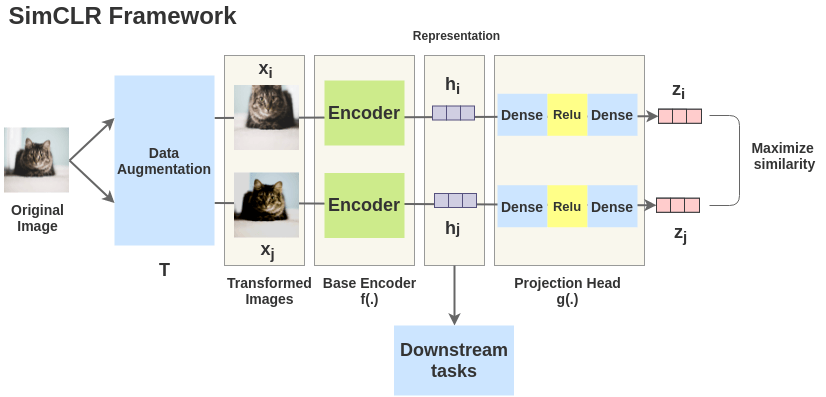
\includegraphics[width=1.0\textwidth]{images/simclr_framework_diagram.png}
	\captionof{figure}{Sơ đồ SimCLR. Hai view của cùng một ảnh được đưa qua encoder và projection head, sau đó tính contrastive loss để tối đa hóa similarity giữa chúng và giảm similarity với các ảnh khác trong batch.}
	\label{fig:simclr_framework}
\end{center}

\subsubsection{MoCo (2020): Thoát khỏi sự Phụ thuộc vào Batch Size}
\label{subsubsec:moco}

\textbf{Momentum Contrast (MoCo)} \cite{He2020} là một cải tiến quan trọng trong contrastive learning, giải quyết nhược điểm lớn của SimCLR: phụ thuộc vào batch size cực lớn.

\textbf{Ý tưởng cốt lõi:}  
Thay vì chỉ sử dụng các negative samples trong mini-batch hiện tại, MoCo duy trì một \textbf{hàng đợi động (queue)} chứa các embedding "key" từ các mini-batch trước đó, mở rộng số lượng negative samples lên hàng chục nghìn.

\textbf{Kiến trúc và cơ chế toán học:}

\begin{itemize}
	\item \textbf{Query Encoder ($f_q$) và Key Encoder ($f_k$):}  
	\[
	q = f_q(x_i), \quad k_+ = f_k(x_j)
	\]  
	Trong đó $x_i, x_j$ là hai view của cùng một ảnh. Các negative keys $k_-$ được lấy từ hàng đợi $Q$.
	
	\item \textbf{Cập nhật Momentum cho Key Encoder:}  
	\[
	\theta_k \leftarrow m \theta_k + (1-m) \theta_q
	\]  
	với $m \in [0.9,0.999]$. Trực giác: các key trong queue không thay đổi đột ngột, đảm bảo sự ổn định khi tính loss contrastive.
	
	\item \textbf{Queue (Dictionary) $Q$:}  
	Hàng đợi giữ các embedding $k$ từ các mini-batch trước. Khi một key mới được tính, key cũ nhất trong queue sẽ bị loại ra (FIFO).
	
	\item \textbf{InfoNCE Loss:}  
	Với query $q$, positive key $k_+$, và negative keys $\{k_-\}$ trong queue:
	\[
	\mathcal{L}_q = - \log \frac{\exp(q \cdot k_+ / \tau)}{\exp(q \cdot k_+ / \tau) + \sum_{k_- \in Q} \exp(q \cdot k_- / \tau)}
	\]  
	Trực giác: Mạng học cách tăng similarity với positive key, đồng thời giảm similarity với tất cả negative keys trong queue.
	
\end{itemize}

\textbf{Trực giác tổng quát:}  
\begin{itemize}
	\item Queue cho phép sử dụng hàng chục nghìn negative samples mà không cần batch size khổng lồ.
	\item Momentum update giữ consistency giữa các embeddings trong queue, tránh "key stale" quá nhanh.
	\item Kết quả là MoCo vừa học hiệu quả vừa tiết kiệm bộ nhớ và phần cứng so với SimCLR.
\end{itemize}

\begin{center}
	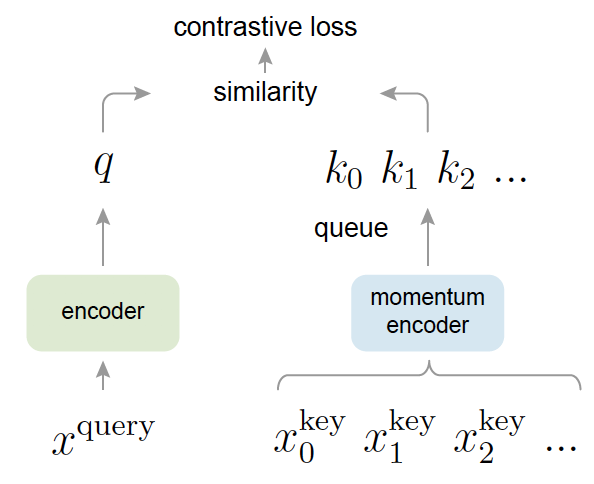
\includegraphics[width=0.9\textwidth]{images/moco_framework_diagram.png}
	\captionof{figure}{Sơ đồ cơ chế MoCo. Query encoder được huấn luyện thông thường, key encoder cập nhật bằng momentum. Queue chứa các negative keys từ các batch trước, mở rộng số lượng negative samples mà không cần batch size lớn.}
	\label{fig:moco_framework}
\end{center}

\subsubsection{Masked Autoencoders (MAE, 2021): Toán học và Trực giác}
\label{subsubsec:mae_math}

\textbf{Ý tưởng cốt lõi:}  
Cho một ảnh $x \in \mathbb{R}^{H \times W \times C}$, chia nó thành $N$ patch $x = [x_1, x_2, \dots, x_N]$. Chọn ngẫu nhiên một tập patch bị che giấu $M \subset \{1,\dots,N\}$ với tỷ lệ masking $\rho$ (ví dụ 75\%). Encoder chỉ nhận các patch \textbf{không bị che}:

\[
x_\text{visible} = \{ x_i \mid i \notin M \}
\]

\textbf{Encoder:}  
\[
h = f_\theta(x_\text{visible})
\]  
với $f_\theta$ là ViT. Biểu diễn $h$ chứa thông tin tiềm ẩn về toàn bộ ảnh.

\textbf{Decoder:}  
Nhận $h$ và các \textbf{mask tokens} $z_m$ cho các patch bị che:
\[
\hat{x}_M = g_\phi(h, z_M)
\]  
với $g_\phi$ là một decoder nhỏ, học để tái tạo các patch bị che.

\textbf{Hàm mất mát:}  
Tái tạo bằng MSE chỉ trên các patch bị che:
\[
\mathcal{L}_\text{MAE} = \frac{1}{|M|} \sum_{i \in M} \| x_i - \hat{x}_i \|_2^2
\]

\textbf{Trực giác:}  
\begin{itemize}
	\item Che giấu phần lớn patch buộc encoder học một biểu diễn \textbf{toàn cục và giàu ngữ nghĩa}, thay vì dựa vào các chi tiết cục bộ.
	\item Decoder chỉ cần nhỏ, vì encoder đã học hầu hết thông tin quan trọng.  
	\item Việc pre-train với MAE giúp encoder nắm được các khái niệm thị giác bậc cao, có thể fine-tune hiệu quả cho các tác vụ downstream như phân loại, phân đoạn, hay detection.
\end{itemize}

\textbf{Điểm nổi bật của MAE:}
\begin{itemize}
	\item Kiến trúc bất đối xứng (encoder lớn, decoder nhỏ) giúp tiết kiệm tính toán.
	\item Tỷ lệ masking cao buộc học biểu diễn toàn cục, tăng khả năng tổng quát.
	\item Thích hợp cho pre-training quy mô lớn trên tập dữ liệu khổng lồ.
\end{itemize}

\begin{center}
	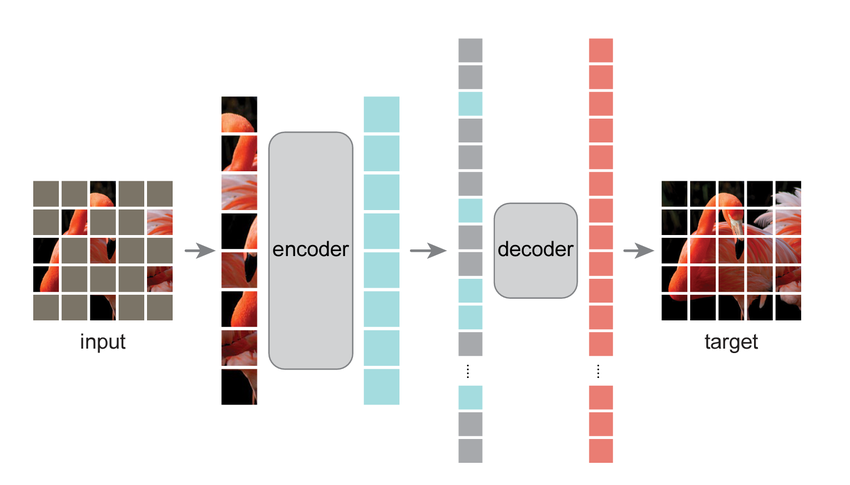
\includegraphics[width=0.9\textwidth]{images/mae_masked_autoencoder_diagram.png}
	\captionof{figure}{Sơ đồ MAE với giải thích trực giác: encoder chỉ nhận patch không bị che, decoder tái tạo patch bị che từ biểu diễn tiềm ẩn và mask tokens.}
	\label{fig:mae_diagram_math}
\end{center}

\subsection{Kết luận và Xu hướng Tương lai}
\label{subsec:ssl_conclusion_trends}
Học Tự giám sát đã thay đổi căn bản cách chúng ta huấn luyện các mô hình thị giác.
\begin{itemize}
	\item \textbf{Học Tương phản} (SimCLR, MoCo) đã chứng minh rằng chúng ta có thể học các biểu diễn mạnh mẽ, có khả năng phân biệt tốt, phù hợp cho các tác vụ như phân loại và tìm kiếm.
	\item \textbf{Học dựa trên Che giấu} (MAE, BEiT) lại xuất sắc trong việc học các biểu diễn giàu ngữ nghĩa và bối cảnh, rất phù hợp để fine-tune cho các tác vụ dày đặc như phát hiện và phân đoạn.
\end{itemize}
Xu hướng hiện nay (2024-2025) đang hướng tới việc \textbf{kết hợp cả hai trường phái}. Các mô hình SOTA như \textbf{DINOv2} và \textbf{iBOT} kết hợp cả tín hiệu tương phản và tín hiệu tái tạo để học được các biểu diễn vừa có tính phân biệt, vừa giàu ngữ nghĩa.

Hơn nữa, SSL chính là công nghệ nền tảng cho phép huấn luyện các \textbf{mô hình nền tảng đa phương thức} như CLIP, DALL-E, và các mô hình thị giác tổng quát như I-JEPA. Bằng cách cho phép máy tính "học như một đứa trẻ"—quan sát thế giới và tự tìm ra các quy luật—SSL đang mở đường cho một thế hệ AI thông minh hơn, tổng quát hơn và ít phụ thuộc vào sự giám sát của con người hơn.

\section*{Tài liệu tham khảo}
\begin{itemize}
	\item[1] Chen, T., Kornblith, S., Norouzi, M., \& Hinton, G. (2020). A simple framework for contrastive learning of visual representations. In \textit{International conference on machine learning (ICML)}. (Paper gốc giới thiệu SimCLR).
	\item[2] He, K., Fan, H., Wu, Y., Xie, S., \& Girshick, R. (2020). Momentum contrast for unsupervised visual representation learning. In \textit{Proceedings of the IEEE/CVF conference on computer vision and pattern recognition (CVPR)}. (Paper gốc giới thiệu MoCo).
	\item[3] He, K., Chen, X., Xie, S., Li, Y., Dollár, P., \& Girshick, R. (2022). Masked autoencoders are scalable vision learners. In \textit{Proceedings of the IEEE/CVF conference on computer vision and pattern recognition (CVPR)}. (Paper gốc giới thiệu MAE).
	\item[4] Grill, J. B., Strub, F., Altché, F., Tallec, C., Richemond, P., Buchatskaya, E., ... \& Valko, M. (2020). Bootstrap your own latent-a new approach to self-supervised learning. In \textit{Advances in Neural Information Processing Systems (NeurIPS)}. (Giới thiệu BYOL, một phương pháp tương phản không cần negative samples).
	\item[5] Bao, H., Dong, L., \& Wei, F. (2021). Beit: Bert pre-training of image transformers. \textit{arXiv preprint arXiv:2106.08254}. (Giới thiệu BEiT, một phương pháp masked image modeling khác).
	\item[6] Caron, M., Touvron, H., Misra, I., Jégou, H., Mairal, J., Bojanowski, P., \& Joulin, A. (2021). Emerging properties in self-supervised vision transformers. In \textit{Proceedings of the IEEE/CVF international conference on computer vision (ICCV)}. (Giới thiệu DINO, một phương pháp SSL dựa trên self-distillation).
\end{itemize}